En este capítulo estudiamos el efecto del ruido en la detección digital. Supongamos que la onda modulada PAM que contiene los símbolos pasa esencialmente sin distorsión por el canal, pero la misma se recibe con ruido adicional $n(t)$:
\begin{equation*}
    y(t) = x(t) + n(t) = \sum_k a_k p(t-kT_s) + n(t)
\end{equation*}
Supongamos además que conocemos (mediante algún mecanismo de sincronización), el momento exacto donde muestrear la onda recibida. El paso final es entonces analizar la muestra recibida (contaminada de ruido) y decidir a qué símbolo pertenece en transmisión. Esto se diagrama en la Figura \ref{fig:deteccion ruido}.

\begin{figure}
    \begin{center}
        \begin{blockdiagram}
            \node at (0,0) (input) {\small $x(t) = \sum_k a_k p(t-kT_s) + n(t)$};
            \node[coordinate, right=2cm of input] (space) {};
            \node[block, right=of space, align=center, inner sep=4pt] (sample) {\begin{circuitikz}\draw (0,0) to[switch] node[ocirc]{} (.8,0);\end{circuitikz}};
            \draw[thick,->] (input) -- (sample);
            \node[block, right =3cm of sample, align=center, label=above:{\small Detector}] (detector) {\begin{tikzpicture} \draw (0,0) -| ++(.3,.3) |- ++(.3,.3); \end{tikzpicture}};
            \draw[thick,->] (sample) --node[midway]{\small $y(kT_s) = a_k+n_k$} (detector);
            \node[right =of detector] (salida) {\small $\hat{a}_k$};
            \draw[thick,->] (detector) -- (salida);
            \node[block, below=of space, align=center] (sincr) {Sincronismo};
            \node[coordinate, left=1cm of sincr] (input_sincr) {};
            \draw[thick,->] (sincr) -| (sample);
            \draw[thick,dashed,->] (input_sincr) -- (sincr);
        \end{blockdiagram}
    \end{center}
    \caption{Onda PAM afectada por ruido y sistema de detección.}\label{fig:deteccion ruido}
\end{figure}

A la entrada del comparador o detector tenemos una muestra $y(kT_s)$. Bajo las hipótesis anteriores, no hay ISI, es decir $x(kT_s) =a_k$ sin error, por lo que tenemos:
\begin{equation*}
    y_k = y(kT_s) = x(kT_s) + n(kT_s) = a_k + n_k
\end{equation*}
es decir el símbolo original perturbado por un ruido aleatorio $n_k:=n(kT_s)$ en el instante de muestreo.

Consideremos que este ruido aleatorio tiene una densidad $f_N(n)$, es decir:
\begin{equation*}
\p{a\leqslant n_k \leqslant b} = \int_a^b f_N(n)dn,
\end{equation*}
tal que:
\begin{align*}
    &\E{n_k} = 0 &\text{ruido centrado}\\
    &\E{n_k^2} = \sigma_N^2 < \infty &\text{potencia finita}.
\end{align*}
Por ahora no discutiremos cómo el ruido $n(t)$ se generó en el canal analógico, pero típicamente será un ruido blanco filtrado en recepción, como veremos más adelante.

\begin{figure}
    \begin{center}
    \begin{tikzpicture}
        \draw [->] (-3,0) -- (3,0) node [anchor=north] {$n$};
        \draw [->] (0,-0.5) -- (0,2.5) node [anchor=west] {$f_N(n)$};
        \draw [teal, thick, domain=-2.5:2.5,samples=200] plot (\x,{2*exp(-1*((\x)^2))});
        \node[align=left] at (8,1.5) {Densidad del ruido\\
        \; -- $\E{n_k}=0$\\\; -- $\mathrm{Var}(n_k) = \E{n_k^2} = \sigma_N^2$};
    \end{tikzpicture}
    \end{center}
    \caption{Ejemplo de densidad de ruido en recepción.}\label{fig:densidad ruido}
\end{figure}

\section{Probabilidad de error de detección para símbolos binarios}

Consideramos primero el caso binario, donde $a_k$ toma dos valores posibles: $A_1 < A_2$. Por ejemplo: $A_1=0, A_2 = A$ en el caso unipolar, y $A_1=-A$, $A_2=A$ en el caso polar. En este caso, la densidad de la variable aleatoria $y_k$ recibida es la densidad de $n_k$ trasladada por el símbolo. Tenemos por tanto $2$ densidades \emph{condicionales} al símbolo enviado,
\begin{gather*}
    f_{Y|A_1} (y) = f_N(y-A_1);\\
    f_{Y|A_2} (y) = f_N(y-A_2).
\end{gather*}
El detector decidirá si el símbolo transmitido fue $A_1$ o $A_2$ \emph{comparando con un umbral} $A_0$ a diseñar:
\begin{gather*}
    y_k < A_0 \Rightarrow \hat{a}_k=A_1, \\
    y_k > A_0 \Rightarrow \hat{a}_k=A_2.
\end{gather*}
Habrá error en la detección ($a_k\neq\hat{a}_k$) si:
\begin{itemize}
    \item $y>A_0$ y se transmitió $A_1$;
    \item $y<A_0$ y se transmitió $A_2$.
\end{itemize}
La probabilidad \emph{condicional al símbolo transmitido} de cada uno de estos eventos se corresponde con las áreas sombreadas en la Figura \ref{fig:ruido deteccion binaria}.

\begin{figure}
    \begin{center}
        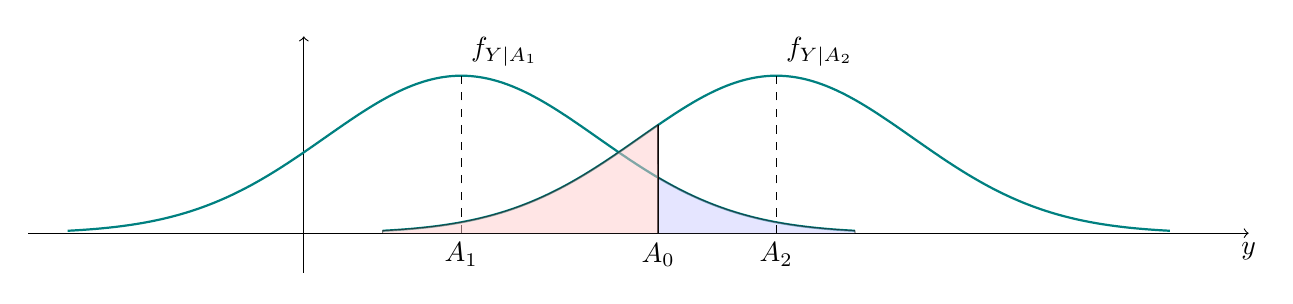
\begin{tikzpicture}
            \draw [->] (-3.5,0) -- (12,0) node [anchor=north] {$y$};
            \draw [->] (0,-0.5) -- (0,2.5);
            \draw [teal, thick, domain=-3:7,samples=200] plot (\x,{2*exp(-1*((\x-2)^2)/6)});
            \draw [dashed] (2,0) node [anchor=north] {$A_1$} -- (2,2) node [anchor=south west] {$f_{Y|A_1}$};
            \draw [domain=4.5:7,samples=200,fill=blue!20,opacity=0.5] (4.5,0) --  plot (\x,{2*exp(-1*((\x-2)^2)/6)}) -- (7,0);
            \begin{scope}[shift={(4,0)}]
                \draw [teal, thick, domain=-3:7,samples=200] plot (\x,{2*exp(-1*((\x-2)^2)/6)});
                \draw [dashed] (2,0) node [anchor=north] {$A_2$} -- (2,2) node [anchor=south west] {$f_{Y|A_2}$};
                \draw [thick] (0.5,0) node [anchor=north] {$A_0$} -- (0.5,{2*exp(-1*(1.5^2)/6)});
                \draw [domain=-3:0.5,samples=200,fill=red!20,opacity=0.5] (-3,0) --  plot (\x,{2*exp(-1*((\x-2)^2)/6)}) -- (0.5,0);
            \end{scope}
        \end{tikzpicture}        
    \end{center}
    \caption{Errores en la detección binaria.}\label{fig:ruido deteccion binaria}
\end{figure}

La probabilidad de error de detección es entonces:
\begin{equation*}
P_e := \p{\text{error}} = \p{\text{error}\mid A_1} \p{a_k=A_1} + \p{\text{error}\mid A_2} \p{a_k=A_2}.
\end{equation*}
Calculemos la probabilidad condicionales de cada evento, indicada en sombreado en la Figura \ref{fig:ruido deteccion binaria}.
\begin{align*}
    P(\text{error}|A_1) &= \int_{A_0}^\infty f_N(y-A_1)dy = \int_{A_0-A_1}^\infty f_N(n) dn;\\
    P(\text{error}|A_2) &= \int_{-\infty}^{A_0} f_N(y-A_2)dy = \int_{-\infty}^{-(A_2-A_0)} f_N(n)dn.\\
\end{align*}
Esta descomposición de ilustra en la Figura \ref{fig:ruido deteccion binaria 2}
\begin{figure}
    \begin{center}
    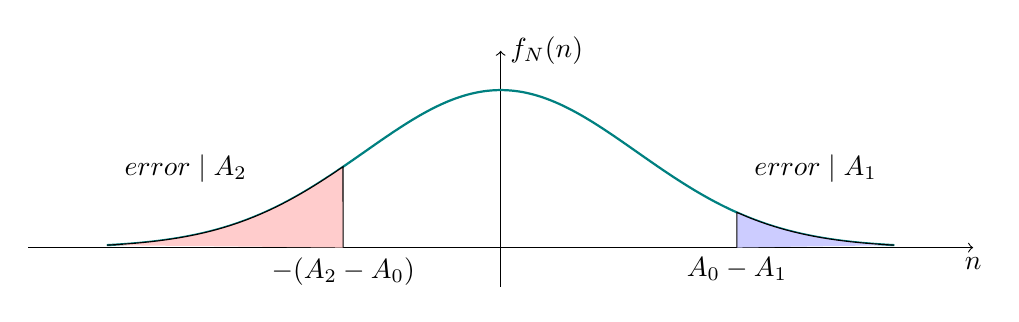
\begin{tikzpicture}
        \draw [->] (-6,0) -- (6,0) node [anchor=north] {$n$};
        \draw [->] (0,-0.5) -- (0,2.5) node [anchor=west] {$f_N(n)$};
        \draw [teal, thick, domain=-5:5,samples=200] plot (\x,{2*exp(-1*((\x)^2)/6)});
        \draw [domain=-5:-2,samples=200,fill=red!20] plot (\x,{2*exp(-1*((\x)^2)/6)}) -- (-2,0) node [anchor=north] {$-(A_2-A_0)$};
        \draw [domain=3:5,samples=200,fill=blue!20] (3,0) node [anchor=north] {$A_0-A_1$} -- plot (\x,{2*exp(-1*((\x)^2)/6)});
        \path (-4,1) node {$\p{\text{error}\mid A_2}$};
        \path (4,1) node {$\p{\text{error}\mid A_1}$};
    \end{tikzpicture}
    \end{center}
    \caption{Probabilidades condicionales de error de detección en términos de la densidad del ruido.}\label{fig:ruido deteccion binaria 2}
\end{figure}

Si subimos el umbral $A_0$, $\p{\text{error}\mid A_1}$ baja pero sube $P\p{\text{error}\mid A_2}$, y viceversa. Entonces hay un compromiso en la elección del umbral. La selección óptima es la que minimiza $P_e$; la hallamos por
diferenciación:
\begin{equation*}
\frac{\partial P_e}{\partial A_0} = - \p{A_1} f_N (A_0 - A_1) + \p{A_2} f_N(A_0 - A_2) = 0
\end{equation*}
Existe $A_0^*$ que anula la derivada, y es tal que:
\begin{equation*}
\frac{\p{A_2}}{\p{A_1}}=\frac{f_N(A_0^*-A_1)}{f_N(A_0^*-A_2)}.    
\end{equation*}

Supongamos además que:
\begin{itemize}
    \item Los símbolos son equiprobables.
    \item El ruido es simétrico, con densidad $f_N(n)$ par y decreciente en $|n|$. El caso típico aquí es la distribución Gaussiana (que es la que se ilustra en la Figura \ref{fig:ruido deteccion binaria 2}).
\end{itemize}

Bajo estas hipótesis adicionales, la condición anterior implica que $f_N(A_0^*-A_1) = f_N(A_0^*-A_2)$. Para que se dé la igualdad, se requiere entonces:
\begin{equation*}
A_2-A_0^* = A_0^*-A_1 \Rightarrow A_0^*=\frac{A_1+A_2}{2},
\end{equation*}
de donde:
\begin{equation}
{\col{P_e= \p{\text{error}|A_1} = \p{\text{error}|A_2} = \int_{\frac{A_2-A_1}{2}}^\infty f_N(n)\d n}}
\end{equation}
Si en cambio, $P(A_2) > P(A_1)$ por ejemplo, entonces $f_N(A_0^*-A_1) > f_N(A_0^*-A_2) \Rightarrow A_0^*-A_1 < A_2-A_0^*$,  es decir, el umbral óptimo se desplaza hacia el símbolo menos probable.

Especialicemos la fórmula anterior al caso más usado: el ruido tiene distribución normal o Gaussiana, de media $0$ y varianza $\sigma_N^2$ como antes. En ese caso:
\begin{equation*}
f_N(n) = \frac{1}{\sqrt{2\pi}\sigma_N}\e^{-\frac{n^2}{2\sigma_N^2}}.
\end{equation*}
En este caso, si $n_k\sim \mathcal{N}(0,\sigma_N^2)$, entonces $n_k/\sigma_N \sim \mathcal{N}(0,1)$ estándar. Utilizando la definición \eqref{eq:def cola gaussiana} para la cola de la distribución normal estándar tenemos que:
\begin{equation}\label{eq:error binario gaussiano}
P_e=\int_{\frac{A_2-A_1}{2}}^\infty f_N(n)\d n = \p{n_k>\frac{A_2-A_1}{2}} = \p{\frac{n_k}{\sigma_N}>\frac{A_2-A_1}{2\sigma_N}} = Q\left(\frac{A_2-A_1}{2\sigma}\right).    
\end{equation}
La función $Q(z)$ como se mencionó está tabulada y disponible en los paquetes de software. Para $z\gg 1$ también vale la aproximación:
\begin{equation*}
    Q(z) \approx \frac{1}{\sqrt{2\pi}z}e^{-\frac{z^2}{2}}.
\end{equation*}

\begin{ejemplo}[Transmisión unipolar binaria y equiprobable con ruido Gaussiano]
Este caso corresponde a elegir $A_1=A$ y $A_2=0$, por lo que $A_0^* = A/2$ y:
\begin{equation*}
    P_e = Q\left(\frac{A}{2\sigma_N}\right)
\end{equation*}
\end{ejemplo}

\begin{ejemplo}[Transmisión polar binaria y equiprobable con ruido Gaussiano]
Este caso corresponde a elegir $A_1=A$ y $A_2=-A$, por lo que $A_0^*=0$ y:
\begin{equation*}
    P_e = Q\left(\frac{A}{\sigma_N}\right)
\end{equation*}
\end{ejemplo}

Notar que en ambos casos, para reducir $P_e$, debo aumentar $\frac{A}{\sigma}$. De hecho, $P_e$ cae muy rápidamente:
\begin{center}
    \begin{tabular}{c|c}
        $\frac{A}{\sigma_N}$ & $Q\left(\frac{A}{\sigma_N}\right)$\\
        \hline
        $2$ & $0.022$\\
        $4$ & $3\times 10^{-5}$\\
        $6$ & $10^{-8}$
    \end{tabular}
\end{center}

El cociente $\frac{A}{\sigma_N}$ está operando como una relación señal a ruido. De hecho, $\sigma_N^2=E[n_k^2]=N$ es la potencia media del ruido. La amplitud $A^2$ está relacionado siempre relacionada con la potencia media de la onda $x(t) = \sum a_k p(t-kT_s)$. La relación exacta depende también del pulso $p(t)$ y el código de línea utilizado. Veamos un ejemplo.

\begin{ejemplo}[Pulsos rectangulares NRZ en ruido Gaussiano]
    Supongamos que utilizamos pulsos NRZ, es decir $p(t)= p_{[0,T_s]}(t)$ NRZ. En este caso, vimos que se cumplía la fórmula simple \eqref{eq:potencia energia pulso simplificada} para la potencia transmitida:
    \begin{equation*}
    \langle x^2 \rangle = \bar{E}_p f_s = \E{a_k^2}\|p\|^2 f_s = \E{a_k^2} f_s T_s = \E{a_k^2}.
    \end{equation*} 
    Tenemos entonces los siguientes casos:
    \begin{description}
        \item[Polar, NRZ:] $\langle x^2 \rangle  = A^2 \Rightarrow \left(\frac{S}{N}\right) = \frac{A^2}{\sigma_N^2}$.
        \item[Unipolar, NRZ:] $\langle x^2 \rangle =\frac{A^2}{2}\Rightarrow \left(\frac{S}{N}\right) = \frac{A^2}{2\sigma_N^2}$.
    \end{description}
    Se deduce entonces que:
    \begin{align*}
        P_e &= Q\left(\sqrt{\frac{S}{N}}\right) &\text{Onda polar NRZ}\\
        P_e &= Q\left(\frac{1}{\sqrt{2}}\sqrt{\frac{S}{N}}\right) &\text{Onda unipolar NRZ}\\
    \end{align*}
    En particular, la onda polar es más eficiente, ya que tiene menor $P_e$ para igual relación señal a ruido.
\end{ejemplo}

\section{Error de detección en un alfabeto $M$-ario}

En este caso, elegimos una ``constelación'' de niveles para representar los $M$ símbolos. Por ejemplo, para $M$ par, elegimos una constelación polar $\{\pm A, \pm 3A,\pm 5A,\ldots,\pm (M-1)A\}$, espaciados $2A$. Para este caso, solo analizaremos la situación en que todos los símbolos son equiprobables y el ruido es Gaussiano, que se presenta en la Figura \ref{fig:ruido m-ario}.

\begin{figure}
    \begin{center}
        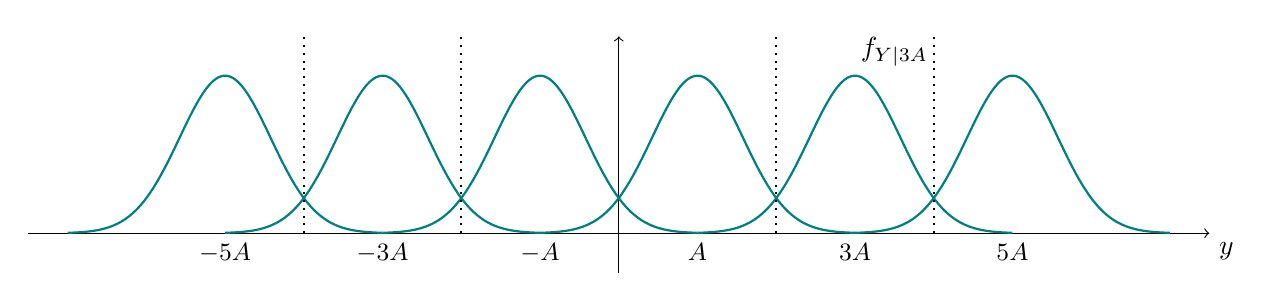
\begin{tikzpicture}
            \draw [->] (-7.5,0) -- (7.5,0) node [below right] {$y$};
            \draw [->] (0,-0.5) -- (0,2.5);
            \foreach \a in {-5,-3,-1,1,3,5} {
                \draw [teal, thick, domain={\a-2}:{\a+2},samples=200] plot (\x,{2*exp(-1.5*((\x-\a)^2))});
            }
            \path (3.5,2) node [anchor=south] {$f_{Y|3A}$};
            
            \node[below] at (-5,0) {\small $-5A$};
            \node[below] at (-3,0) {\small $-3A$};
            \node[below] at (-1,0) {\small $-A$};
            \node[below] at (1,0) {\small $A$};
            \node[below] at (3,0) {\small $3 A$};
            \node[below] at (5,0) {\small $5 A$};

            \foreach \a in {-4,-2,2,4} {
                \draw [dotted,thick] (\a,0) -- (\a,2.5);
            }
        \end{tikzpicture}
    \end{center}
    \caption{Densidades condicionales y umbrales de detección en un alfabeto $M$-ario equiespaciado.}\label{fig:ruido m-ario}
\end{figure}

Resulta intuitivo de la Figura \ref{fig:ruido m-ario} que los umbrales de detección óptimos son los puntos intermedios entre los símbolos de la constelación, $0,\pm 2A, \pm 4A,\ldots$. En este caso, para todos los símbolos intermedios se tiene que:
\begin{equation*}
    \p{\text{error} \mid a_k=l} = \p{|n|>A} = 2\p{n>A} = 2Q\left(\frac{A}{\sigma_N}\right) \quad l=\pm A,\ldots, (M-3)A.
\end{equation*}
Para los símbolos extremos:
\begin{equation*}
    \p{\text{error} \mid a_k=\pm (M-1)A} = \p{n>A} = Q\left(\frac{A}{\sigma_N}\right)
\end{equation*}

Por lo tanto se tiene que:
\begin{equation}\label{eq:error polar m-ario gaussiano}
    P_{e,\text{símbolo}}:=\p{\text{error}} = (M-2) \frac{1}{M} 2Q\left(\frac{A}{\sigma_N}\right) + \frac{1}{M}2Q\left(\frac{A}{\sigma_N}\right) = 2\left(\frac{M-1}{M}\right)Q\left(\frac{A}{\sigma_N}\right)
\end{equation}
Notar que la probabilidad anterior es la probabilidad de \emph{error de símbolo}, es decir, de detectar un símbolo que no es el transmitido. Sin embargo, aquí no necesariamente coincide con la probabilidad de \emph{error de bit} ya que cada símbolo codifica varios bits.

Nuevamente $A/\sigma_N$ juega el rol de una relación señal a ruido, como lo ilustra el siguiente Ejemplo.

\begin{ejemplo}[Pulsos rectangulares NRZ, alfabeto $M$-ario y ruido Gaussiano]
    Nuevamente utilizamos la fórmula simplificada \eqref{eq:potencia energia pulso simplificada} para obtener:
    \begin{equation*}
        S := \langle x^2 \rangle = \bar{E}_p f_s = \E{a_k^2} ||p||^2 f_s = \E{a_k^2}.
    \end{equation*}
    Calculando:
    \begin{equation*}
    \E{a_k^2}=A^2\frac{2}{M}\left(1+3^2+5^2+\cdots+(M-1)^2\right) = \frac{2A^2}{M}\left(\frac{M^3-M}{6}\right) = \frac{A^2(M^2-1)}{3},
    \end{equation*}
    donde se utilizó arriba una fórmula para la suma de los cuadrados de los números impares. La relación señal a ruido resulta entonces en:
    \begin{equation*}
        \left(\frac{S}{N}\right)=\frac{A^2}{\sigma^2}\left(\frac{M^2-1}{3}\right),
    \end{equation*}
    y la probabilidad de error de decodificación de símbolo queda:
    \begin{equation}\label{eq:prob error simbolo m-ario}
        {\col{P_e=2\left(\frac{M-1}{M}\right)Q\left(\sqrt{\frac{3}{M^2-1}\left(\frac{S}{N}\right)}\right)}.}
    \end{equation}

    \textbf{Observación: }para la misma relación señal a ruido, aumentar el número de símbolos \emph{incrementa} la probabilidad de error, a cambio de transmitir a una mayor $\vti$.
\end{ejemplo}

Para finalizar esta sección, volvamos a la discusión entre \emph{error de símbolo} y \emph{error de bit}. En el caso binario no hay diferencia, pero en el caso $M-$ario hemos calculado la probabilidad de error de símbolo. Sin embargo, a la hora de comparar diferentes mecanismos de transmisión, es mejor expresar las tasas de error en términos de bits. Para ello definimos:
\begin{definicion}
    Se denomina \emph{Bit Error Rate (BER)} a la tasa de bits erróneos sobre la tasa de bits transmitidos por el canal.
\end{definicion}

La tasa de bits transmitidos por el canal es precisamente la $\vti=f_s \log_2 M$, siendo el caso más común el que $M$ es potencia de $2$. La tasa de bits erróneos es igual a la frecuencia de símbolo $f_s$ por la probabilidad de error de símbolo $P_{e,\textrm{simbolo}}$ por la cantidad media de bits equivocados en cada símbolo.

Como la función $Q(z)$ decae muy rápidamente, la probabilidad de error de símbolo está fuertemente concentrada solo en los símbolos adyacentes. Por lo tanto, podemos despreciar la probabilidad de error de símbolo a los no adyacentes. Además, para símbolos adyacentes podemos asignar los bits utilizando \href{https://en.wikipedia.org/wiki/Gray_code}{codificación de Gray}. Con este mecanismo, ilustrado en el Cuadro \ref{tabla:codigo gray} para el caso $M=8$, los símbolos adyacentes difieren en un único bit, por lo que la cantidad de bits erróneos al equivocar un símbolo es aproximadamente $1$, si despreciamos los errores a símbolos no adyacentes. Con este razonamiento llegamos a:
\begin{equation*}
\textrm{BER} \approx \frac{P_{e,\text{símbolo}}}{\log_2 M}.
\end{equation*}
siendo $P_{e,\text{símbolo}}$ la calculada en \eqref{eq:error polar m-ario gaussiano}.

\begin{table}
    \begin{center}
        \begin{tabular}{|c|c|}
            \hline
            \textbf{Nivel} & \textbf{Símbolo} \\ \hline
            $7A$ & $010$\\
            $5A$ & $011$\\
            $3A$ & $001$\\
            $A$  & $000$\\
            $-A$ & $100$\\
            $-3A$ & $101$\\
            $-5A$ & $111$\\
            $-7A$ & $110$ \\ \hline
        \end{tabular}
    \end{center}
    \caption{Código de Gray para $M=8$ símbolos, es decir $3$ bits. Los códigos adyacentes difieren en un único bit.}\label{tabla:codigo gray}
\end{table}

\section{Detección digital en un canal con ruido blanco Gaussiano}

Apliquemos ahora lo visto anteriormente al caso práctico en que la señal digital PAM se envía por un canal de ancho de banda acotado, el cual introduce ruido blanco Gaussiano. Para limitar el ruido es necesario, al igual que en la comunicación analógica, colocar un filtro de recepción, antes de pasar a la etapa de detección estudiada anteriormente. El esquema general es el que de ilustra en la Figura \ref{fig:deteccion canal ruido}. Tenemos entonces tres ondas PAM:
\begin{itemize}
\item $x_T(t)= \sum_k a_k p_T(t-kT_s)$, la onda transmitida. $p_T(t)$ es la forma de pulso del transmisor.
\item $x(t)=\sum a_k p(t-kT_s)$, la onda a la salida del canal, a la que se superpone el ruido blanco Gaussiano $w(t)$ de densidad espectral $\eta_0/2$. La forma de pulso $p(t)$ incorpora la distorsión del canal.
\item $x_R(t) = \sum_k a_k p_R(t-kT_s)$, la onda a la salida del filtro de recepción, afectada del ruido filtrado $n(t)$.
\end{itemize}

\begin{figure}
    \begin{center}
        \begin{blockdiagram}
            \node at (0,0) (input) {\small $x_T(t)$};
            \node[block, right =of input, align=center] (canal) {\pasabajos{B}{.5}};
            \draw[thick, ->] (input) -- (canal);
            \node[circle, draw, thick, right=of canal] (add) {$+$}; 
            \node[above=of add] (ruido) {\small $w(t)$};
            \draw[thick, ->] (canal) -- (add);
            \draw[thick, ->] (ruido) -- (add);
            \begin{scope}[on background layer]
                \node[draw, rectangle, dashed, fill=gray!15!white, fit=(canal) (ruido) (add), inner sep=5pt,label=above:Canal] {};
            \end{scope}
            \node[block, right =2.6cm of add, align=center, inner sep=8pt, label=above:{\small Filtro Rx}] (rx) {$\hat{H}_r$};
            \draw[thick, ->] (add) -- node[midway,above]{{\small $x(t)+w(t)$}} (rx);
            \node[below=of rx] (sincr_input) {};
            \node[block, right =.5cm of sincr_input, align=center] (sincr) {Sincronismo};
            \draw[thick, dashed, ->] (sincr_input) -- (sincr);
            \node[block, right =2.2cm of rx, align=center, inner sep=4pt] (sample) {\begin{circuitikz}\draw (0,0) to[switch] node[ocirc]{} (.8,0);\end{circuitikz}};
            \draw[thick, ->] (rx) -- node[midway,above]{\small $x_R(t)+n(t)$} (sample);
            \draw[thick,->] (sincr) -| (sample);
            \node[block, right =of sample, align=center, label=above:{\small Detector}] (detector) {\begin{tikzpicture} \draw (0,0) -| ++(.3,.3) |- ++(.3,.3); \end{tikzpicture}};
            \node[right =of detector] (salida) {\small $\hat{a}_k$};
            \node[above=1cm of sample] (top) {};
            \draw[thick,->] (sample) --node[midway]{\small $y_k$} (detector);
            \draw[thick,->] (detector) -- (salida);
            \begin{scope}[on background layer]
                \node[draw, rectangle, dashed, fill=gray!15!white, fit=(rx) (sincr_input) (sincr) (sample) (detector) (top), inner sep=10pt,label=above:Receptor digital] {};
            \end{scope}            
        \end{blockdiagram}
    \end{center}
    \caption{Transmisión digital sobre un canal ideal de ancho $B$ con ruido aditivo blanco y Gaussiano.}\label{fig:deteccion canal ruido}
\end{figure}

Comencemos analizando el ruido filtrado: utilizando \eqref{eq:espectro filtrado}, éste tiene media nula y
varianza
\begin{equation}\label{eq:varianza ruido filtrado}
\sigma_N^2=\E{n(t)^2}=\frac{\eta_0}{2}\int_{-\infty}^{\infty}|\hat{H}_R(f)|^2 df.    
\end{equation}

Estudiamos ahora varios ejemplos del sistema completo distinguiendo según la forma de pulso transmitida y el filtro de recepción elegido.

\begin{ejemplo}[Pulsos de Nyquist ideales]

    Una primera aproximación sería utilizar como $p_T(t)$ pulsos ideales, con $f_s=2B$, por lo que:
    \begin{equation*}
        p_T(t) = \sinc(\pi f_s t) = \sinc(\pi 2B t) \fourier \hat{P}_T(f) = T_s p_{\left[-\frac{f_s}{2},\frac{f_s}{2}\right]}(f) = T_s p_{[-B,B]}(f).
    \end{equation*}
    En este caso, la señal $x(t)=x_T(t)$ pasa sin distorsión por el canal y solo se adiciona ruido. Tiene sentido entonces colocar como filtro de recepción otro pasabajos ideal $\hat{H}_R(f) = p_{[-B,B]}(f)$ por lo que, utilizando \eqref{eq:varianza ruido filtrado}, $\sigma_N^2 = \eta_0 B$.

    Supongamos ahora que los símbolos $\{a_k\}$ son independientes con media $\mu$ y varianza $\sigma_a^2$, la densidad espectral de potencia de $x_T(t)=x(t)$ es:

    \begin{center}
    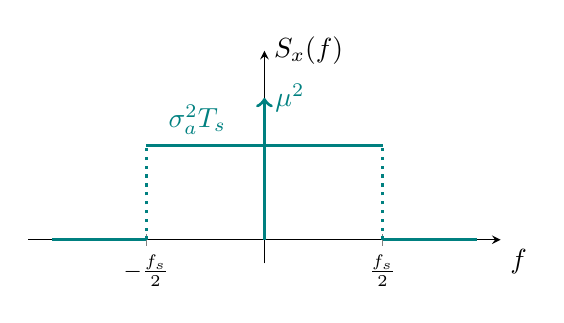
\begin{tikzpicture}
            \begin{axis}[ x=1.5cm, y=1.5cm, axis lines=middle,  
                every x tick label/.append style={font=\footnotesize},
                every y tick label/.append style={anchor=south east},
                xlabel=$f$,
                x label style={anchor=north west},
                ylabel=$S_x(f)$,
                y label style={anchor=west},
                xmin=-2,xmax=2,ymin=-.2,ymax=1.6,
                ytick=\empty,
                xtick = {-1,1},
                xticklabels = {$-\frac{f_s}{2}$,$\frac{f_s}{2}$},
                clip=false,
                ]
                \addplot[teal, very thick, domain=-1:1, samples=10] {.8} node[midway,above left, xshift=-1em] {$\sigma_a^2 T_s$};
                \addplot[teal, very thick, domain=-1.8:-1, samples=10] {0};
                \addplot[teal, very thick, domain=1:1.8, samples=10] {0};
                \draw[dotted, teal, very thick] (axis cs:-1,0) -- (axis cs:-1,.8);
                \draw[dotted, teal, very thick] (axis cs:1,0) -- (axis cs:1,.8);
                \draw[->, teal, very thick] (axis cs:0,0) -- (axis cs:0,1.2) node[right] {$\mu^2$};
            \end{axis}
    \end{tikzpicture}
    \end{center}

    Integrando $S_x$ se obtiene la potencia transmitida:
    \begin{equation*}
        S:=\langle x^2 \rangle = \int_{-\infty}^\infty S_x(f)df = \mu^2+\sigma_a^2 = \E{a_k^2}.
    \end{equation*}
    En particular, como $||p||^2 = T_s$ (calcularla en frecuencia), se verifica en este caso también que:
    \begin{equation*}
        S:=\langle x^2 \rangle = \E{a_k^2} ||p||^2 f_s = \bar{E}_p f_s.
    \end{equation*}

    Tenemos entonces una potencia transmitida $S=\bar{E}_p f_s = \E{a_k^2}$ y una potencia de ruido $N:=\sigma_N^2=\eta_0 B = \eta_0 f_s/2$. Calculamos la probabilidad de error:
    \begin{description}
        \item[Caso polar binario: ] $a_k = \pm A$, $A_0^*=0$, $S=A^2$ y utilizando \eqref{eq:error binario gaussiano}:
        \begin{equation*}
            P_e = Q\left(\frac{A}{\sigma_N}\right) = Q\left(\sqrt{\frac{S}{N}}\right).
        \end{equation*}
        Observar que coincide con la expresión para pulsos NRZ. Otra expresión posible es surge de observar que:
        \begin{equation*}
            S = \bar{E}_p f_s , \quad N=\eta_0 \frac{f_s}{2} \Longrightarrow P_e = Q\left(\sqrt{\frac{2\bar{E}_p}{\eta_0}}\right),
        \end{equation*}
        una expresión que solo depende de parámetros físicos del canal (energía de pulso, densidad del ruido). En particular \emph{no depende de la frecuencia de señalización}.

        \item[Caso unipolar binario: ]  Se procede igual que en el caso anterior, tomando $a_k=\{0,A\}$ de donde $A_0^* =A/2$, $\mu=A/2$ y $\sigma_a^2 = A^2/4$. La potencia transmitida en este caso es $S=\bar{E}_p f_s = A^2/2$. Utilizando nuevamente \eqref{eq:error binario gaussiano}:
        \begin{equation*}
            P_e = Q\left(\frac{A}{2\sigma_N}\right) = Q\left(\frac{1}{\sqrt{2}}\sqrt{\frac{S}{N}}\right).
        \end{equation*}
        O bien en términos de la energía de pulso y la densidad del ruido:
        \begin{equation*}
            P_e = Q\left(\sqrt{\frac{\bar{E}_p}{\eta_0}}\right),
        \end{equation*}
        que deja claro que esta señalización es menos eficiente en potencia para el mismo BER.
    \end{description}
\end{ejemplo}


\begin{ejemplo}[Pulsos de Nyquist no ideales]
    
    En este caso, el pulso tiene un exceso de ancho de banda $\alpha$ respecto a $f_s/2$. Se plantea entonces la disyuntiva: dejamos pasar el pulso intacto (controlando así la ISI) o elegimos un filtro más restrictivo. Analicemos por ahora el primer caso, es decir, tomemos $f_s$ tal que:
    \begin{equation*}
        \frac{f_2}{2}(1+\alpha) = B,
    \end{equation*}
    para que el pulso pase intacto, y utilicemos como antes un pasabajos ideal en recepción de ancho $B$. En particular ahora la potencia del ruido es mayor para la misma frecuencia de símbolo:
    \begin{equation*}
        N := \sigma_N^2 = \eta_0 B = \frac{\eta_0f_s}{2}(1+\alpha).
    \end{equation*}

    En este caso, la fórmula simple de energía de pulso $S=\bar{E}_p f_s$ no es válida, por lo que es difícil calcular la potencia media transmitida $S$ para cualquier alfabeto. En cambio, trabajaremos directamente con la energía media del pulso transmitido, que se calcula como:
    \begin{equation*}
        \bar{E}_p := \E{a_k^2}||p||^2 = \E{a_k^2}T_s \underbrace{\left(f_s \int_{-\infty}^\infty |\hat{P}(f)|^2df\right)}_{\beta} = \beta \E{a_k^2} T_s,
    \end{equation*}
    siendo $\beta$ un parámetro que depende de la forma del pulso. En particular se tiene, utilizando la desigualdad de Cauchy-Schwarz:
    \begin{equation*}
        \underbrace{\left(\int_{-(1+\alpha)\frac{f_s}{2}}^{(1+\alpha)\frac{f_s}{2}} \hat{P}(f)df\right)^2}_{=p(0)^2=1} \leqslant \left(\int_{-(1+\alpha)\frac{f_s}{2}}^{(1+\alpha)\frac{f_s}{2}} |\hat{P}(f)|^2 df\right) \underbrace{\left(\int_{-(1+\alpha)\frac{f_s}{2}}^{(1+\alpha)\frac{f_s}{2}} 1 df\right)}_{=f_s(1+\alpha)}.
    \end{equation*}
    De aquí deducimos que $\beta(1+\alpha)\geqslant 1$. Es fácil ver que además $\beta\leqslant 1$, con igualdad en ambos casos para el pulso de Nyquist ideal, $\alpha=0$.

    Tomemos entonces como ejemplo el caso polar binario, $\bar{E}_p = \beta A^2 T_s$, de donde podemos escribir $A=\sqrt{\frac{\bar{E}_p f_s}{\beta}}$. Utilizando nuevamente el umbral $0$ y la fórmula \eqref{eq:error binario gaussiano} queda:
    \begin{equation*}
        P_e = Q\left(\frac{A}{\sigma_N}\right) = Q\left(\sqrt{\frac{2\bar{E}_p}{\eta_0 (1+\alpha)\beta}}\right).
    \end{equation*}
    Como el factor $\beta(1+\alpha)\geqslant 1$, se aumenta la probabilidad de error. La explicación intuitiva es que, para evitar la ISI, el pulso tiene simetría vestigial y por lo tanto menos potencia en la parte alta de la banda, lo que hace que el filtro de recepción ideal introduzca ruido en exceso. Se plantea entonces la pregunta de si no podemos hacer algo mejor, lo cual veremos en la Sección \ref{sec:filtro acoplado}. Algo análogo ocurre en el caso unipolar.
\end{ejemplo}


\begin{ejemplo}[Pulsos rectangulares]
    Supongamos ahora que el ancho de banda del canal no es un inconveniente, $B$ es suficientemente grande respecto a la frecuencia de símbolo $f_s$, por lo que podemos usar pulsos rectangulares. De todos formas, debemos agregar un filtro en recepción para reducir el ruido blanco Gaussiano. Se plantea entonces el siguiente dilema:
    \begin{itemize}
        \item Si el ancho de banda de $\hat{H}_R$ es muy ancho, los pulsos no se deforman, la ISI es menor, pero la etapa de detección tiene más ruido.
        \item Si el filtro $\hat{H}_R$ es angosto, se reduce el ruido pero los pulsos se deforman, introduciendo ISI no deseada.
    \end{itemize}
    Estos dos efectos se ilustran en la Figura \ref{fig:nrz ruido}. Aquí se utilizan pulsos NRZ con $f_s=4\unit{\kilo\hertz}$ y se varía el ancho de banda del filtro de recepción desde $.5f_s$ a $4f_s$. Como puede verse, el ojo se abre a medida que más lóbulos se dejan pasar por el filtro, mejorando la ISI, pero introduciendo cada vez más ruido.

    \begin{figure}
        \begin{center}
        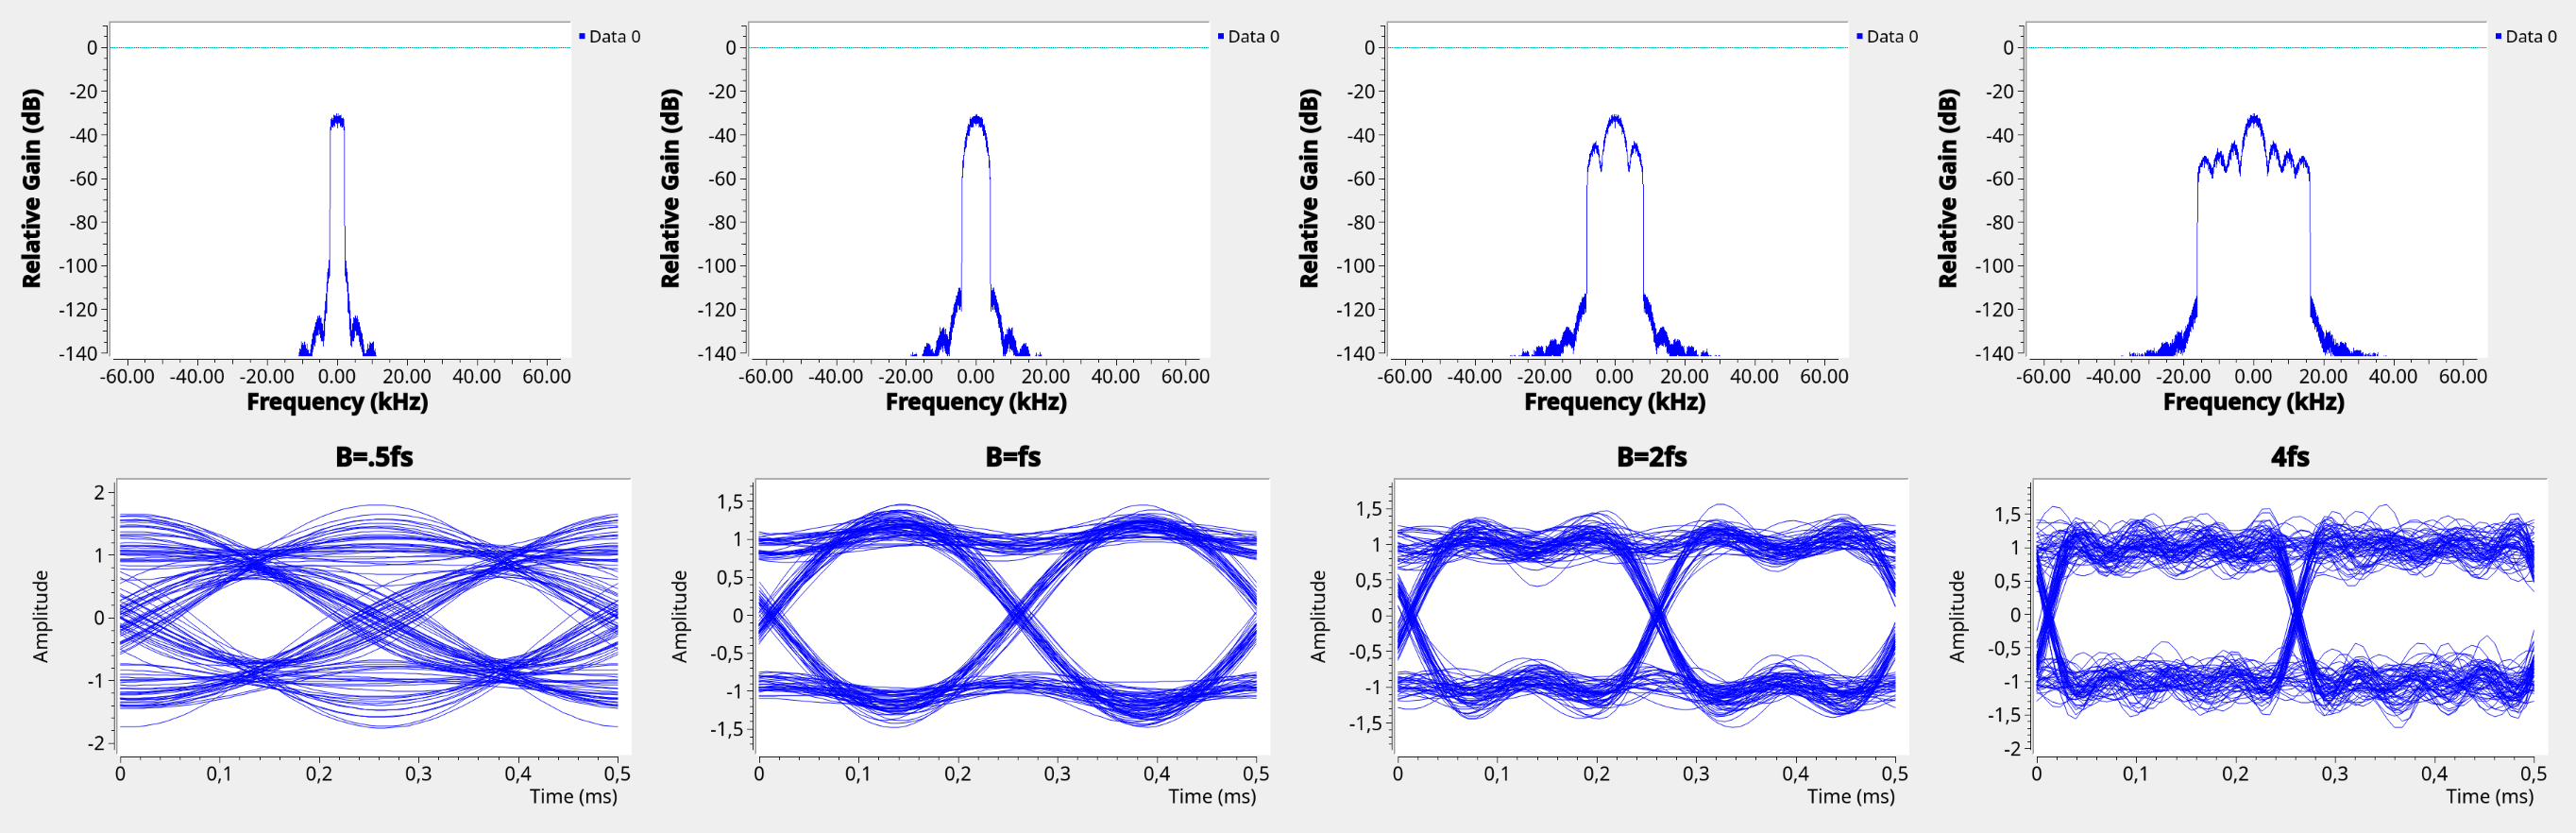
\includegraphics[width=\textwidth]{figuras/pulso_NRZ_ruido_filtrado.png}
        \end{center}
        \caption{Espectro y diagramas de ojo de pulsos NRZ polares afectados de ruido con diferentes filtros de recepción A medida que aumenta el ancho de banda, disminuye la ISI pero aumenta el ruido.}\label{fig:nrz ruido}
    \end{figure}
    
\end{ejemplo}

La observación crucial es la siguiente: el filtro de recepción no tiene por qué ser un pasabajos ideal, es parte del diseño del sistema. A la luz entonces de los últimos dos ejemplos, surge naturalmente la siguiente pregunta: ¿es posible diseñar un filtro que maximice la relación $A/\sigma_N$ en el instante de detección? Esto permite minimizar la probabilidad de error debida al ruido. Esto lleva al \emph{filtro acoplado} que analizamos a continuación.

\section{Detección óptima en presencia de ruido: filtro acoplado}\label{sec:filtro acoplado}

Replanteamos el problema del diseño del filtro de recepción $H_R$ (denotado aquí por $H$ por simplicidad) buscando la mínima probabilidad de error debida al ruido, ignorando por ahora la ISI. En vez de ``dejar pasar'' la señal, permitimos que el pulso se distorsione en el filtro de recepción, pero con el objetivo de que \emph{en el momento de muestreo el pulso de salida tenga amplitud máxima en relación al ruido}.

Para analizar esto, inevitablemente debemos analizar cómo afecta el filtro al pulso transmitido: concentrémonos en un único símbolo en $t=0$, donde se transmite $a_0 p(t)$ siendo $p(t)$ un pulso arbitrario, pero conocido y de energía finita. Dicho pulso se contamina con ruido blanco Gaussiano de densidad espectral $\eta_0/2$. Por ahora $a_0$ es cualquier símbolo (polar, unipolar, $M$-ario, etc.).

Sea entonces $\hat{H}(f)$ la respuesta en frecuencia del filtro de recepción a diseñar, y $h(t)$ su respuesta impulsiva. La señal observada a la salida de $\hat{H}$ será entonces:
\begin{equation*}
    y(t) = x_R(t) + n(t) = a_0 (p*h)(t) + n(t)
\end{equation*}
donde $n(t)$ es un ruido de media $0$ y varianza dada por \eqref{eq:varianza ruido filtrado}:
\begin{equation*}
    \sigma_N^2 = \frac{\eta_0}{2}\int_{-\infty}^\infty |\hat{H}(f)|^2df
\end{equation*}
La señal $y(t)$ se muestrea en un cierto tiempo $\tau$ a definir, obteniendo:
\begin{equation*}
    y_k = A' + n(\tau) = a_0 (p*h) (\tau) + n(\tau),
\end{equation*}
donde el valor $A'$ depende tanto de $a_0$ (ej: $\pm A$) como de la deformación del pulso. Como vimos, la probabilidad de error en detección es mínima cuanto mayor sea el cociente $A'/\sigma_N$, que por lo anterior verifica:
\begin{equation}\label{eq:filtro acoplado 1}
    \left(\frac{A'}{\sigma_N}\right)^2 = \frac{2 a_0^2}{\eta_0}\frac{|(p*h)(\tau)|^2}{\int_{-\infty}^{+\infty} |\hat{H}(f)|^2 df}.
\end{equation}

Buscamos entonces $h \fourier \hat{H}$ para maximizar lo anterior, de modo de minimizar la probabilidad de error. Sin embargo, esto no es inmediato ya que el filtro $H$ aparece en el numerador (en forma de su respuesta impulsiva) y denominador (a través de su respuesta en frecuencia). Para simplificar en algo la expresión anterior conviene pasar primero a frecuencia
\begin{equation*}
    (p * h) \fourier \hat{P}(f) \hat{H}(f) \quad \Longrightarrow \quad (p * h)(\tau) = \int_{-\infty}^{+\infty} \hat{P}(f)
\hat{H}(f) \e^{j2\pi f \tau}d f,
\end{equation*}
donde en la segunda parte usamos la transformada inversa de Fourier.

El objetivo del problema puede escribirse entonces, sustituyendo en la ecuación \eqref{eq:filtro acoplado 1}, cómo:
\begin{equation}\label{eq:filtro acoplado 2}
    \max_{\hat{H}(f)} \frac{\left|\int_{-\infty}^{+\infty}
\hat{P}(f) \hat{H}(f) \e^{j2\pi f \tau}df\right|^2}{\int_{-\infty}^{+\infty} |\hat{H}(f)|^2 df}.
\end{equation}

La optimización anterior en principio es \emph{en todos los posibles filtros}, por lo cual su solución no es trivial. Sin embargo, podemos apelar nuevamente a la desigualdad de Cauchy-Schwarz (compleja):
\begin{equation*}
\left|\int \hat{V}(f) \overline{\hat{W}(f)}df\right|^2\leqslant \int_{-\infty}^{+\infty} |\hat{V}(f)|^2 df \int_{-\infty}^{+\infty} |\hat{W}(f)|^2 df,
\end{equation*}
con igualdad $\Leftrightarrow \hat{V} = K \hat{W}$.

Tomemos entonces $\hat{V}(f) = \hat{H}(f)$ y $\overline{\hat{W}(f)} = \hat{P}(f)\e^{j2\pi f \tau}$. Usando la desigualdad tenemos:
\begin{equation*}
\left|\int_{-\infty}^{+\infty} \hat{P}(f) \hat{H}(f) \e^{j2\pi f \tau} df\right|^2\leqslant \int_{-\infty}^{+\infty} |\hat{H}(f)|^2 df \int_{-\infty}^{+\infty} |\hat{P}(f)|^2 df,
\end{equation*}
de donde:
\begin{equation*}
    \frac{\left|\int_{-\infty}^{+\infty} \hat{P}(f) \hat{H}(f) \e^{j2\pi f \tau}  df\right|^2}{\int_{-\infty}^{+\infty} |\hat{H}(f)|^2 df} \leqslant \int_{-\infty}^{+\infty} |\hat{P}(f)|^2 df = ||p||^2.
\end{equation*}

Por lo tanto, el máximo en \eqref{eq:filtro acoplado 2} es acotado, y la igualdad se alcanza si y sólo si:
\begin{equation*}
\hat{H}(f) = K\overline{\hat{P}(f)}\e^{-j2\pi f \tau} \Rightarrow h(t)=K
p\left(-(t-\tau)\right)\Rightarrow \col{h(t) = K p(\tau-t)}.    
\end{equation*}

\begin{figure}[htb]
    \begin{center}
    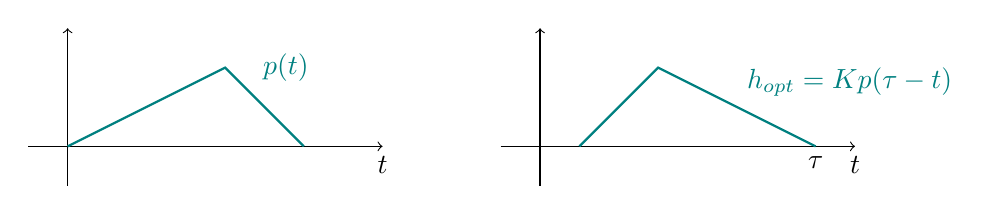
\begin{tikzpicture}
        \draw[->] (-0.5,0) -- (4,0) node [anchor=north] {$t$};
        \draw[->] (0,-0.5) -- (0,1.5);
        \draw[teal,thick] (0,0) -- (2,1) node[right,xshift=1em] {$p(t)$} -- (3,0);
        
        \begin{scope}[shift={(6,0)}]
                \draw[->] (-0.5,0) -- (4,0) node [anchor=north] {$t$};
                \draw[->] (0,-0.5) -- (0,1.5);
                \draw[teal,thick] (0.5,0) -- (1.5,1) -- node[above right]{$h_{opt} = K p(\tau - t)$} (3.5,0) node [anchor=north, black] {$\tau$};
        \end{scope}
    \end{tikzpicture}
    \end{center}
    \caption{Filtro acoplado para un pulso genérico $p(t)$.}\label{fig:filtro acoplado}
\end{figure}

Concluimos que la respuesta impulsiva del filtro óptimo tiene la exactamente la forma del pulso incidente, invertido en el tiempo: se dice que el filtro óptimo está \emph{acoplado (o apareado, matched)}  al pulso.

Para interpretar el resultado en el dominio del tiempo, conviene escribir el pulso de salida $p_R =h* p$ para el filtro óptimo:
\begin{align*}
            p_R(t) = (h\ast p) (t)  & = \int_{-\infty}^{+\infty} h(t-\sigma) p (\sigma)\d \sigma\\
            & = K \int_{-\infty}^{+\infty} p(\tau - t + \sigma) p (\sigma)d \sigma \\ & = K r_p(t - \tau).
\end{align*}
Aquí $r_p(\cdot)$ es la autocorrelación del pulso como señal de cuadrado integrable. Como la autocorrelación es máxima en cero, el pulso de salida toma su amplitud máxima en el instante de muestreo $t=\tau$. En otras palabras: el detector basado en este filtro y muestreo en $t=\tau$ está \emph{correlacionando} la señal de entrada $a_0 p(t) + n(t)$ con la forma de onda conocida del pulso. El momento de máxima correlación se alcanza en el instante de muestreo y es lo que maximiza la amplitud observada respecto al ruido.

Algunas observaciones:
\begin{enumerate}
    \item La constante $K$ es arbitraria, escalar el filtro no cambia el cociente de \eqref{eq:filtro acoplado 2}, ya que amplifica tanto la señal como el ruido. Una elección cómoda es $K=\frac{1}{||p||^2}=\frac{1}{r_p(0)}$: de ese modo el pulso de salida $p_R(t)$ tiene valor máximo igual a $1$, alcanzado en $t=\tau$. En ese caso la amplitud $A'$ de muestreo coincide con la amplitud $a_0$ del símbolo de entrada.
    \item El retardo $\tau$ sería idealmente arbitrario, pero se trata de elegir lo menor posible. La limitante es que, en la práctica queremos $h(t)$ causal, cuando en general $p(-t)$ no lo es. Si el pulso es de duración acotada, se toma $\tau$ igual a la duración del pulso $p(t)$. Si es de duración no acotada (ej: pulso de Nyquist $p(t)=\sinc(\pi f_s t)$), hay que truncarlo.
\end{enumerate}

Volviendo a la ecuación \eqref{eq:filtro acoplado 1}, el máximo de nuestro problema de optimización es $\|p\|^2$. Por lo tanto tenemos:
\begin{equation}\label{eq:snr filtro acoplado}
\col{\left(\frac{A'}{\sigma_N}\right)^2_{\text{max}} = 2 \frac{a_0^2}{\eta_0} ||p||^2.}
\end{equation}

A partir de esta fórmula podemos escribir la probabilidad de error en términos de la energía media del pulso recibido, $\bar{E}_p = E[a_k^2] ||p||^2$, en los distintos casos:
\begin{description}
    \item[Polar binario]
    \begin{equation*}
       \bar{E}_p = A^2 ||p||^2 \Rightarrow \left(\frac{A'}{\sigma_N}\right)_\text{max} = \sqrt{\frac{2\bar{E}_p}{\eta_0}} \Rightarrow P_e^\text{opt} = Q\left(\sqrt{\frac{2\bar{E}_p}{\eta_0}}\right).
    \end{equation*}
    \item[Unipolar binario]
    \begin{equation*}
       \bar{E}_p = \frac{A^2}{2} ||p||^2 \Rightarrow \left(\frac{A'}{\sigma_N}\right)_\text{max} = 2\sqrt{\frac{\bar{E}_p}{\eta_0}} \Rightarrow P_e^\text{opt} = Q\left(\sqrt{\frac{\bar{E}_p}{\eta_0}}\right),
    \end{equation*}
    donde en este caso se usó que el umbral óptimo es $\frac{A}{2\sigma_N}$.
\end{description}

Estas fórmulas son iguales a las que obtuvimos para la detección cuando se utilizan pulsos de Nyquist ideales. Esto no es casualidad, precisamente el filtro acoplado al pulso de Nyquist es el filtro pasabajos ideal. Es decir que en ese caso, filtrar el ruido fuera de banda es lo óptimo. Pero las fórmulas anteriores valen para cualquier forma de pulso con su detector apareado.

\subsection*{Caso M-ario polar} Ya se vio anteriormente que aquí la
probabilidad de error de símbolo es $P_e=2\frac{M-1}{M}
Q\left(\frac{A}{\sigma}\right)$. O sea que también aquí debemos
maximizar $\frac{A}{\sigma}$ y por tanto obtenemos el mismo filtro
acoplado. Escribimos la expresión en términos de $\overline{E}_p$
para este caso:
\begin{gather*}
 E[a_k]^2 = \frac{A^2 (M^2-1)}{3} \Rightarrow \overline{E}_p = A^2 \frac{(M^2-1)}{3}||p||^2
\Rightarrow \left(\frac{A'}{\sigma}\right)^2_{max} = \frac{6 \bar{E}_p}{\eta (M^2-1)}\\
\Rightarrow {\col{P_e^{opt} = 2\frac{M-1}{M}
Q\left(\sqrt{\frac{6\bar{E}_p}{\eta(M^2-1)}}\right)}}
\end{gather*}

\subsection*{Detector acoplado para pulsos rectangulares}

Tomemos por ejemplo los pulsos NRZ, $p(t) = p_{[0,T_s]}(t)$. El
filtro acoplado tendrá la respuesta impulsiva (tomando
$\tau=T_s$):
\[
\Rightarrow h(t) = \dfrac{1}{||p||^2} p(T_s-t) =
\dfrac{1}{T_s}p(t).
\]
\begin{minipage}{0.6\textwidth}
 A la salida del filtro se obtiene el pulso triangular
 \[p_R(t)=h(t)\ast p(t). \]
\end{minipage}
\begin{minipage}{0.4\textwidth}
 \begin{center}
  \bpgf{Imagenes/filAc/filAc-2}
    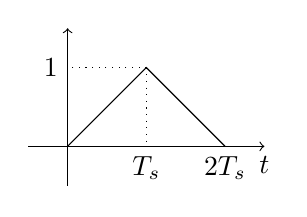
\begin{tikzpicture}
      \draw [->] (-0.5,0) -- (2.5,0) node [anchor=north] {$t$};
      \draw [->] (0,-0.5) -- (0,1.5);
      \draw (0,0) -- (1,1) -- (2,0) node [anchor=north] {$2T_s$};
      \draw [dotted] (1,1) -- (0,1) node [anchor=east] {$1$};
      \draw [dotted] (1,1) -- (1,0) node [anchor=north] {$T_s$};
    \end{tikzpicture}
  \endpgfgraphicnamed
 \end{center}
\end{minipage}

El filtro de recepción distorsionó fuertemente el pulso, pero esto
se  hizo de modo de maximizar $\frac{A}{\sigma}$ en el instante de
$t=T_s$ de muestreo.


\subsection*{¿Qué paso con la ISI?}

Al estudiar un solo pulso aislado, no contemplamos este tema.
Veamos:
\begin{itemize}
 \item En el caso pulsos de Nyquist ideales el detector acoplado es un pasabajos ideal, entonces los pulsos pasan intactos,
 sin ISI.
 \item En el caso de pulsos rectangluares NRZ. Vemos que $p_R(k T_s) = 0$ excepto en un valor ($k=1$). Entonces tampoco hay
 ISI.  Simplemente hay un retardo de $\tau = T_s$ al detectar.
 \item  De hecho, cualquier pulso de duración $\leq T_s$ (por ej., RZ) genera una $p_R(t)$ de duración $\leq
 2T_s$, que debidamente muestreado no genera  ISI.
\end{itemize}


\subsection*{Para pulsos de Nyquist con exceso de ancho de banda
$\alpha$}

El detector acoplado tiene respuesta en frecuencia
\begin{gather*}
 \hat{H}(f) = K \overline{\hat{P}(f)} \e^{-j2\pi f\tau}\\
 \Rightarrow \hat{P}_R = \hat{H}\hat{P} = K |\hat{P}(f)|^2 \e^{-j2\pi f \tau}
\end{gather*}
El último término es un retardo, afecta sólo el instante de
muestreo. A efectos de estudiar la ISI podemos tomar $P_R(f) =
K|\hat{P}(f)|^2$.
\begin{figure}[htb]
 \begin{center}\begin{minipage}{\textwidth}
  \bpgf{Imagenes/filAc/filAc-3}
  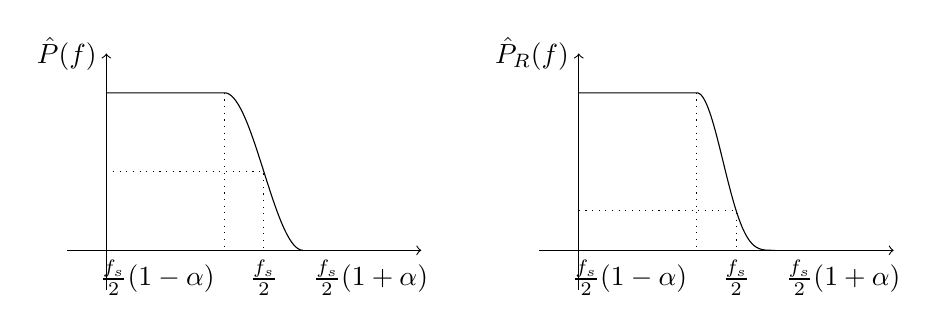
\begin{tikzpicture}
    \draw [->] (-0.5,0) -- (4,0);
    \draw [->] (0,-0.5) -- (0,2.5) node [anchor=east] {$\hat{P}(f)$};
    \draw  (0,2) -- (1.5,2) -- plot  [domain=1.5:2.5,samples=200] (\x,{cos(pi*(\x-1.5) r)+1});
    \draw [dotted] (1.5,2) -- (1.5,0) node [below left] {$\frac{f_s}{2}(1-\alpha)$};
    \draw [dotted] (0,1) -- (2,1) -- (2,0) node [below] {$\frac{f_s}{2}$};
    \path (2.5,0) node [below right] {$\frac{f_s}{2}(1+\alpha)$};
    \begin{scope}[shift={(6,0)}]
    \draw [->] (-0.5,0) -- (4,0);
    \draw [->] (0,-0.5) -- (0,2.5) node [anchor=east] {$\hat{P}_R(f)$};
    \draw  (0,2) -- (1.5,2) -- plot  [domain=1.5:2.5,samples=200] (\x,{(cos(pi*(\x-1.5) r)+1)^2/2});
    \draw [dotted] (1.5,2) -- (1.5,0) node [below left] {$\frac{f_s}{2}(1-\alpha)$};
    \draw [dotted] (0,0.5) -- (2,0.5) -- (2,0) node [below] {$\frac{f_s}{2}$};
    \path (2.5,0) node [below right] {$\frac{f_s}{2}(1+\alpha)$};
    \end{scope}
   \end{tikzpicture}
   \endpgfgraphicnamed\end{minipage}
 \end{center}

\end{figure}

$|\hat{P}(f)|^2$ no tiene simetría, entonces no cumple la condición de ISI nula.

O sea: poner el filtro óptimo desde el punto de vista del ruido,
me complica la ISI.

Alternativas:
\begin{enumerate}
 \item En vez del $H_{opt}$, poner un pasabajos $(1+\alpha)\frac{f_s}{2}$, como ya se estudió. La $P_e$ da un poco peor,
 pero no introduzco ISI que sería más grave.
 \item Sabiendo que va a haber un filtro apareado, diseño $\hat{P}(f)$ para que $|\hat{P}(f)|^2$ no tenga ISI.
 Se usa a veces el pulso de {\bf raíz de coseno alzado.}
\end{enumerate}

% \subsection*{Resumen: comunicación digital banda base}
% \begin{figure}[htb]
%     \centering
%     \resizebox{\textwidth}{!}{%
%     \bpgf{Imagenes/digBB/digBB-1}
    \begin{blockdiagram}
        \matrix[row sep=5mm, column sep=10mm]{
            & & \node[etiqueta] (ruido) {\large ruido blanco, $\frac{\eta}{2}$}; & & & & & \node[punto] (p1) {}; & \node [punto] (p2) {};\\
            \node[etiqueta] (inicio) {\large  $\sum_k a_k p_T(t-kT_s)$}; %& \node[block] (pulso) {$P_T(t)$};
             & \node[block] (canal) {\large CANAL} node[above=3mm] {
                    \begin{minipage}{2.2cm}
                       \large  (ancho de banda $B$)
                    \end{minipage}};
            & \node[operator] (sum) {$+$}; & \node [block] (filtro) {\large $\hat{H}_R(f)$} node [below=5mm] {
            \begin{minipage}{2.5cm}
                FILTRO DE\\RECEPCI�N
                \end{minipage}};
            & \node[punto] (p3) {} node [anchor=south] {\large $x_R(t)+n(t)$}; & \node [punto] (p4) {}; & & & \node[punto] (p5) {}; & \node [draw, isosceles triangle,thick] (comp) {
            \begin{minipage}{5mm}
                $+$\\$-$
            \end{minipage}};
            & \node[etiqueta] (salida) {\large $\{\hat{a}_k\}$};\\
            & & & & & & \node[block] (sinc) {\large SINCR}; & & \node [etiqueta] (v0) {$A_0$};\\
        };
        \draw [-stealth] (inicio) -- (canal);
        \draw [-stealth] (canal) -- (sum);
        \draw [-stealth] (ruido) -- (sum);
        \draw [-stealth] (sum) -- (filtro);
        \draw (filtro) -- (p3) -- (p4) -- (p2);
        \draw [-stealth] (p3) |- (sinc);
        \draw [-stealth] (sinc) -| (p1);
        \draw [-stealth] (p5) |- (comp.150);
        \draw [-stealth] (v0) |- (comp.south west);
        \draw [-stealth] (comp) -- (salida);
    \end{blockdiagram}
\endpgfgraphicnamed

%     }
% \end{figure}
% \FloatBarrier

% \begin{itemize}
%  \item Transmito sucesión de pulsos $\sum a_k p_T(t-kT_s)$ (PAM)
%  \item El canal introduce 2 distorsiones
% \begin{enumerate}
%   \renewcommand{\theenumi}{\roman{enumi}}
%   \item \label{itemRes:1}Forma del pulso, por filtrado. Puede causar ISI.

%   \item \label{itemRes:2}Ruido blanco.
% \end{enumerate}
% \end{itemize}

% Si nos concentramos en (\ref{itemRes:1}), elegimos un pulso de
% Nyquist y/o colocamos un \emph{ecualizador} en $\hat{H}_R(f)$.

% Si nos concentramos en (\ref{itemRes:2}), ponemos en
% $\hat{H}_R(f)$ el \emph{detector acoplado}.

% Hay dos casos extremos en que las dos funciones se realizan
% simultaneamente:

% \begin{itemize}
%  \item $p(t) = \sinc(\pi f_s t)$ (Nyquist ideal), $\hat{H}_R(f)$ pasabajos ideal. Se aplica a la situación:
%     \begin{itemize}
%      \item canal con $B$ muy restrictiva.
%      \item puedo implementar la complejidad de pulsos/filtro.
%     \end{itemize}
%  \item $p(t)$ rectángular NRZ o RZ. Detector acoplado: $h_R(t) = \frac{1}{T_s}p(t)$. Se aplica a la situación:
% \begin{itemize}
%  \item $B$ muy grande (respecto a $f_s$).
%   \item Implementación más simple. Sobre todo, el amplificador de transmisión puede ser no lineal.
% \end{itemize}
% \end{itemize}

% En otros casos, puede existir conflicto entre los objetivos de
% combatir las distorsiones (\ref{itemRes:1}) y (\ref{itemRes:2}).
% Por ejemplo se vio que esto ocurría al usar pulsos de Nyquist con
% exceso de ancho de banda. Aquí o se realiza un diseño conjunto de
% $p_T$, $\hat{H}_R$, o sino se acepta una detección subóptima
% respecto al ruido.

\section{Repetidores regenerativos}

Supongamos se transmite una onda digital de banda base por un
cable largo. Al propagarse la onda se introduce atenuación, que
debe compensarse por amplificación posterior. Una estrategia
comúnmente usada es dividir el cable en tramos y amplificar en
cada tramo. Ejemplo de uso: cajas subterráneas en telefonía.

\begin{figure}
 \begin{center}
    \begin{blockdiagram}
    \matrix[row sep=5mm, column sep=10mm]{
        & \node[etiqueta] (ruido1) {$n_1$}; & & \node[etiqueta] (ruido2) {$n_2$}; & & & \node[etiqueta] (ruidom) {$n_m$};\\
        \node[etiqueta] (inicio) {$x(t)$}; & \node[operator] (sum1) {$+$}; & \node[block] (amp1) {AMP}  node [above right=5mm] {$y_1(t)$} node [below=3mm] {\begin{minipage}{1.5cm}\centering ganancia\\ $\frac{1}{a}$\end{minipage}}; & \node[operator] (sum2) {$+$}; & \node[block] (amp2) {AMP}; & \node[etiqueta] (puntos) {$\ldots$}; & \node[operator] (summ) {$+$}; & \node[block] (ampm) {AMP}; & \node[etiqueta] (salida) {$y(t)$};\\
    };
    \draw [->,ultra thick] (inicio) -- node [anchor=north] {\begin{minipage}{20mm}\centering TR.1\\ atenuación $a$ ($a\ll 1$)\end{minipage}} (sum1);
    \draw [->] (sum1) -- (amp1);
    \draw [->] (ruido1) -- (sum1);
    \draw [->,ultra thick] (amp1) -- node [anchor=north] {TR. 2} (sum2);
    \draw [->] (ruido2) -- (sum2);
    \draw [->] (sum2) -- (amp2);
    \draw [->,ultra thick] (amp2) -- (puntos);
    \draw [->,ultra thick] (puntos) -- (summ);
    \draw [->] (ruidom) -- (summ);
    \draw [->] (summ) -- (ampm);
    \draw [->] (ampm) -- (salida);
  \end{blockdiagram}
 \end{center}
 \caption{Repetidor regenerativo}\label{fig:repetidor regenerativo}
\end{figure}

Suponemos que cada etapa tiene ruido aleatorio de varianza
$E[n_i^2] = \sigma^2$.

\[y_1 = \frac{1}{a}(a x + n_1) = x+ \frac{n_1}{a} \qquad \Longrightarrow \left(\frac{S}{N}\right)_1 =
\frac{\langle x^2 \rangle}{\frac{\langle n_1^2\rangle}{a^2}} = a^2
\frac{\langle x^2\rangle}{\sigma^2}.\]

Para la segunda etapa:
\[y_2 = \frac{1}{a}(a y_1 +n_2) = y_1 + \frac{n_2}{a} = x + \frac{n_1+n_2}{a}.\]

Por el mismo razonamiento,
\[y(t) = y_m(t) = x(t) + \frac{n_1+n_2+\cdots+n_m}{a}.\]

\begin{align*}
 \left(\frac{S}{N}\right)_m & = \frac{\langle x^2 \rangle}{\frac{1}{a^2} E\left[(n_1+n_2+\cdots+n_m)^2\right]} =
  \frac{a^2 \langle x^2\rangle}{m \sigma^2}, \qquad \text{suponiendo ruidos independientes.}
%\Rightarrow                   & =
\end{align*}
\[{\col{ \left(\frac{S}{N}\right)_m = \frac{1}{m}
\left(\frac{S}{N}\right)_1}}\]

 Vemos que la relación señal-ruido se degrada linealmente en $m$. Por lo tanto
la $P_e$ se degrada fuertemente (por ejemplo,
$P_e=Q\left(\sqrt{\frac{S}{N}}\right)$ para el caso polar, con
pulsos ideales).

\begin{ejemplo}[numérico] Señal polar, $\left(\frac{S}{N}\right)_1 = 100 \  (20\,dB)$, $m=20$
repetidores.
  \[ \Rightarrow \left(\frac{S}{N}\right)_m = 5 \Rightarrow P_e  = Q(\sqrt{5}) = 1.29\cdot 10^{-2}, \quad\text{muy alto.}\]
 \end{ejemplo}

\subsection*{Repetidor regenerativo}

En vez de solo amplificar (señal y ruido), realiza una detección y
regenera la señal PAM. Sea $p$ la probabilidad de error de una
etapa, $p=Q\left(\sqrt{\left(\frac{S}{N}\right)_1}\right)$.

Suponemos $p\ll 1$ y errores independientes en cada etapa.
Calculamos la probabilidad de error de $m$ etapas. Notar que
\[1 - P_e(m\text{ etapas})  = (1-P_e(1 \text{ etapa}))^m \]
(es decir, para no tener errores en un símbolo exijo no tenerlos
en ninguna de las $m$ detecciones independientes). Por tanto
\[P_e(m\text{ etapas}) = 1 -(1-p)^m  \approx 1-(1-mp) = mp.\]
En este caso, $P_e$ se deteriora linealmente con $m$.

Volviendo al ejemplo, $p=Q(10) = 7.7\cdot 10^{-24}$ para una
etapa, por tanto
\[ P_e (20 \text{ etapas}) \approx 20 p = 1.5\cdot 10^{-22},\]
muchísimo más bajo que en el caso no regenerativo.

\paragraph{Moraleja}$\phantom{1}$
\begin{itemize}
 \item Es mejor regenerar.
 \item Esta es una de las mayores ventajas de la comunicación digital por sobre la analógica.
\end{itemize}
